\documentclass{article}

\usepackage[fleqn]{amsmath}
\usepackage{amssymb}
\usepackage{hyperref}
\usepackage{url}
\usepackage{graphicx}
\usepackage{geometry}
\usepackage{babel}
\usepackage{enumitem}
\usepackage{parskip}
\usepackage{chemfig}
\usepackage{pdfpages}
\usepackage{xcolor}
\usepackage{tikz}
\usepackage{fancybox}
\usepackage{makecell}
\usepackage{pgfplots}
\usepackage{soul}
\usepackage{ulem}
\usepackage{wrapfig}
\usepackage{subcaption}
\usepackage[T1]{fontenc}
\usepackage{esvect}
\usetikzlibrary{arrows}
\usetikzlibrary{decorations.pathreplacing}
\pgfplotsset{compat=1.17}

\geometry{
    a4paper,
    total={170mm, 257mm},
    left=20mm,
    top=20mm
}

\hypersetup{
    colorlinks=true,
    linkcolor=black,
    urlcolor=blue,
    pdftitle={Environmental chemistry and biology}
}

\newcommand{\figbox}[1]{ 
    \begin{figure*}[ht!]        
        \begin{center}            
            \fbox{#1}        
        \end{center}    
    \end{figure*}
}

\newcommand{\wrapfill}{
    \par
    \ifnum \value{WF@wrappedlines} > 0
        \addtocounter{WF@wrappedlines}{-1}%
        \null\vspace{
            \arabic{WF@wrappedlines}
            \baselineskip
        }
        \WFclear
    \fi
    \phantom{}
}

\newcommand{\cfig}[1]{%
  \begin{figure*}[ht!]%
    \centering%
    #1%
  \end{figure*}%
}

\newcommand{\difference}{\,\backslash\,}
\newcommand{\rem}{\underline{Remark}: }
\newcommand{\nots}{\underline{Notation}: }
\newcommand{\prf}{\underline{Proof}: }
\newcommand{\exs}{\underline{Example}: }
\newcommand{\defs}{\underline{Definition}: }
\newcommand{\wrn}{\underline{Warning}: }
\newcommand{\sht}{\ |\ }
\newcommand{\pph}[1]{\paragraph{#1}\phantom{}\\}


% === TEXT ===
\title{\textbf{Environmental chemistry and biology \\ HSLU, Semester 1}}
\author{Matteo Frongillo}

\begin{document}

\maketitle
\tableofcontents
\pagebreak

\part*{Preamble (Week 0)}
\section{Learning objectives}
We should be able to:
\begin{itemize}
    \item define the term ``Environment'';
    \item define the term ``Environmental chemistry'';
    \item define the term ``Environmental biology'';
    \item know the physical and chemical properties,
        defining the environemntal behavior of a substance;
    \item apply the concept of partitioning to analyze and understan
        the behavior of an organic substance in the environment, with
        the provided values.
\end{itemize}

\newpage
\section{Introduction SW 0}
\subsection{Definitions}
\subsubsection{Environmental Chemistry}
Environmental chemistry is the discipline that describes the \textbf{origin,
transport, reactions, effects and fate} of chemical species in the
hydro-, atmo-, geo-, bio- and anthrosphere.

\cfig{\includegraphics*[width=.9\textwidth]{media/env-chemistry.png}}

\subsubsection{Enviromental Biology}
Environmental biology is the study of \textbf{the relationships between
living organisms and their environment}, including the impacts of
human activities.

\begin{center}
    \vspace*{0.25cm}
    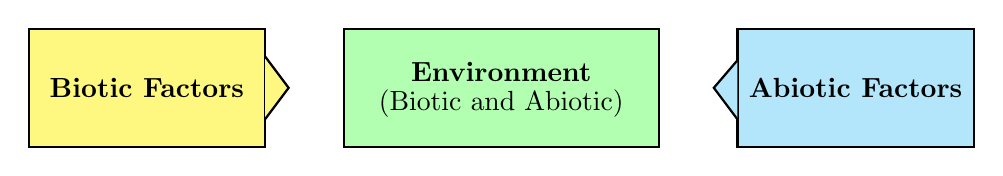
\begin{tikzpicture}
        \draw[fill=yellow!50, draw=black, thick] (0,0) rectangle (3,1.5);
        \draw[fill=yellow!50, draw=black, thick] (3,0.35) -- (3.3,0.75) -- (3,1.15);
        \node at (1.5,0.75) {\textbf{Biotic Factors}};
        
        \draw[fill=green!30, draw=black, thick] 
          (4,0) rectangle (8,1.5);
        \node at (6,0.95) {\textbf{Environment}};
        \node at (6,0.55) {(Biotic and Abiotic)};
        
        \draw[fill=cyan!30, draw=black, thick] (9,0) rectangle (12,1.5);
        \draw[fill=cyan!30, draw=black, thick] (9,0.35) -- (8.7,0.75) -- (9,1.1);
        \node at (10.5,0.75) {\textbf{Abiotic Factors}};
    \end{tikzpicture}
\end{center}

In an ecosystem, biotic factors include all living organisms and
microorganisms. These organisms interact through predation, competition,
and sysmbiosis, forming a complex web of life.\\
Abiotic factors, lie water, sunlight, temperature, pH levels, and
minerals, influence the biotic components.

Human activities, such as the introduction of radioactive wastes, can
disrupt the balance by altering the chemistry of the environment and
harming living organisms.

\subsection{Chemical structure and Environmental behavior}
We consider two groups of properties of chemicals:
\subsubsection{Physical properties}
\begin{itemize}
    \item Vapor pressure (mp, bp);
    \item Solubility (H$_2$O, ...);
    \item Acid / Base strength (pK$_a$, pK$_b$);
    \item Partition coefficients (e.g. K$_{OW}$).
\end{itemize}

These properties describe \textbf{Dispersion} in different compartments $\Rightarrow$ Mobility and Toxicity.

\subsubsection{Chemical properties $\rightarrow$ Reactivity}
\begin{itemize}
    \item Functional groups (-OH, -NH$_2$, ...);
    \item Electronic substituent effects (push/pull of electrons);
    \item Reaction mechanisms.
\end{itemize}

These properties describe \textbf{Transformation} of products $\Rightarrow$ Degradation

\subsection{Partitioning of organic substances in the environment}
The partitioning is the passage of an organic substance from one environmental
compartment to another.\\ It's a physical process and does not involve a chemical reaction:


\setlength{\intextsep}{0pt}%
\begin{wrapfigure}{r}{.55\textwidth}
    \vspace*{1.5cm}
    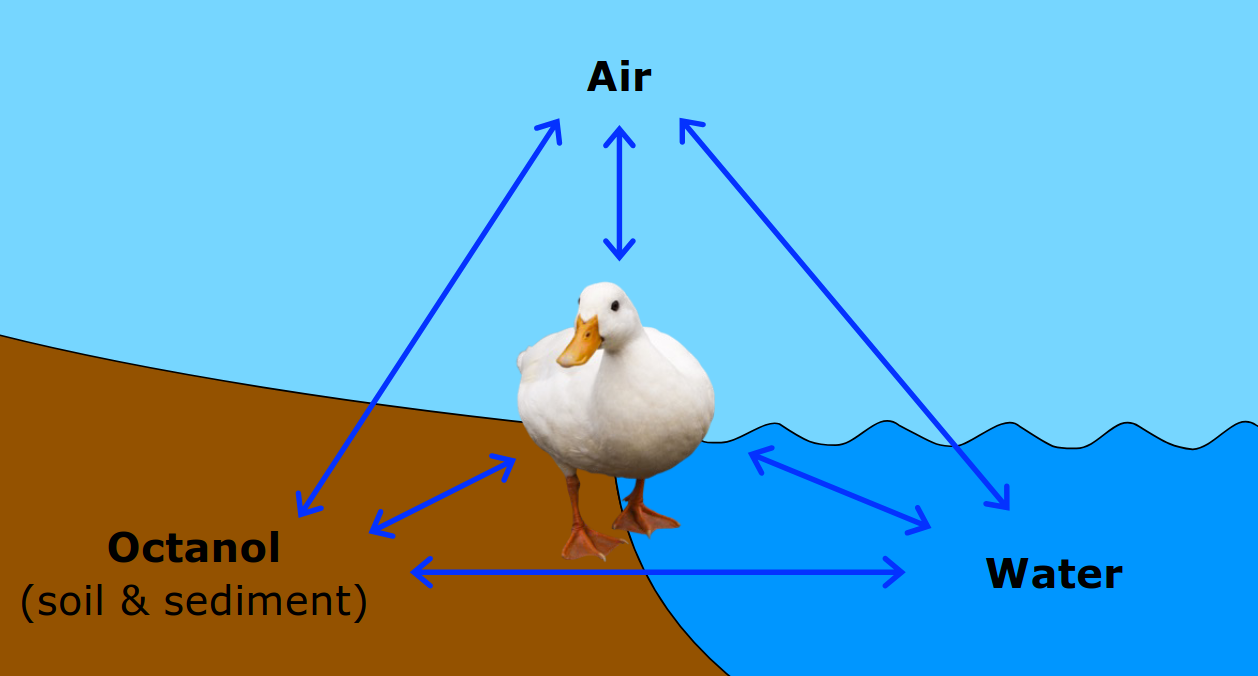
\includegraphics[width=.55\textwidth]{media/partitioning.png}
\end{wrapfigure}

\phantom{}

\begin{enumerate}
    \item air $\longleftrightarrow$ water:
        \begin{itemize}
            \item volatility / vapor pressure;
            \item water solubility;
        \end{itemize}
    \item water $\longleftrightarrow$ soil:
        \begin{itemize}
            \item adsorption (sticking to particles);
            \item water solubility;
        \end{itemize}
    \item soil $\longleftrightarrow$ air:
        \begin{itemize}
            \item adsorption;
            \item volatility / vapor pressure;
        \end{itemize}
    \item all phases $\longleftrightarrow$ biota:
        \begin{itemize}
            \item lipophilicity (fat solubility).
        \end{itemize}
\end{enumerate}
\wrapfill
\vspace*{-3cm}

\subsection{Chemical transformations under environmental conditions}
There are two fundamental pathways:

\subsubsection{Abiotic}
In compartments Air, Water, Soil $\rightarrow$ \textbf{Energy source: temperature, light}
\begin{enumerate}
    \item Hydrolysis: water breaks down a compound;
    \item Oxidation: process where a substance loses electrons, often involving oxygen;
    \item Reduction: process where a substance gains electrons, often involving the breakdown of pollutant in low-oxygen conditions;
    \item Photochemical reactions: reaction driven by sunlight, where light energy breaks down chemicals.
\end{enumerate}

\subsubsection{Biotic}
In organisms $\rightarrow$ \textbf{Catalyst: enzymes}
\begin{enumerate}
    \item Oxidation: enzymes help break down organic molecules within organisms;
    \item Reduction: in organisms, reduction reactions often involve energy production, such as anaerobic environments;
    \item Hydrolysis: enzymes within organisms facilitate hydrolysis to break down larger molecules, like proteins or carbohydrates;
    \item Secundary reactions: additional reactions that happen following primary processes.
\end{enumerate}

\subsection{Biological transformations}
\subsubsection{Abiotic transformations}
\begin{itemize}
    \item These occur in the non-living components of the environment.\\
        Energy for these transformations often comes from higher
        temperatures or sunlight;
    \item Photochemical reactions are particularly important in
        atmosphere, driven by sunlight. They can lead to the breakdown
        of pollutant, through some compounds like PCBs (polychlorinated biphenyls)
        are resistant to degradation, causing persistance in the environment.
\end{itemize}

\subsubsection{Biotic transformations}
\begin{itemize}
    \item These occur within living organisms and are often enzyme-driven;
    \item Persistent pollutants like PCBs, biotic transformations tend
        to be slow, leading to accumulation in organisms. This results
        in \textbf{bioaccumulation} up the foodchain.
\end{itemize}

\newpage
\part{Week 1}
\section{Learning objectives}
We should be able to:
\begin{itemize}
    \item provide for at least 5 of the 8 primary sources of pollutants;
    \item apply the 5-key aspects of a pollutant to predict its behaviour in the environemnt;
    \item discuss how pollutants move through different environmental compartments;
    \item briefly describe with one example the pollutant categories;
    \item recognize the pollutant classes by their Lewis structure;
    \item compare and contrast the similarities and differences among various pollutant categories,
        including their sources, chemical properties, environmental impact, and persistence.
\end{itemize}

\newpage
\section{Anthrosphere and Environmental impact}
\pph{Definition:}
The anthrosphere is the part of the environment that's \textbf{made
or operated by humans}. The anthrosphere is where \textbf{pollutants are made} and
from which they are released with profound effect on all other environmental spheres.

It also strongly affected by pollutants, e.g. acid rains, which cause deterioration of
stone structures and corrosion of metal components.

\pph{Impact:}
It is essential to view the anthrosphere as a distinct environmental sphere,
when considering environmental chemistry and sustainability. Just a look around
us shows the dwellings, buildings, roads, factories, power lines, and numerous
other things constructed and operated by human as a visible evidence of the
existence of the anthrosphere of Earth.

\subsection{Human primary sources}
\cfig{\includegraphics*[width=.8\textwidth]{media/anthrosphere.png}}
\begin{enumerate}
    \item Industrial activities: factories, mining and processing plants release air,
        water, and soil pollutants (SO$_2$, NO$_x$, PM, VOCs), including
        chemicals and heavy metals (Hg);
    \item Transportation: vehicles and ships emit harmful gases (CO$_2$, CO, NO$_x$),
        and particulate matter, contibuting to air pollution and climate change;
    \item Agriculture: farming activities generate pollutants such as pesticides (Glyphosate, Atrazin),
        fertilizers (NH$_3$), and methane (CH$_3$), leading to water contamination
        and greenhouse gas emissions;
    \item Energy production: burning fossil fuels for energy emits CO$_2$, SO$_2$,
        and other pollutants, driving air pollution and global warming;
    \item Urban development: construction and waste management in cities produce dust,
        noise, and runoff pollution, impacting air and water quality;
    \item Deforestation and Land Use changes: clearing forests releases CO$_2$ and
        causes soil erosion, contributing to climate change, habitat and biodiversity loss;
    \item Household activities: residential heating, cooking, and consumer products
        emit indoor and outdoor air pollutants like VOCs and particulate matter;
    \item Waterwaste and Sewage: inadequate treatment of sewage and industrial wastewater
        pollutes water bodies with pathogens, nutrients (PO$_4^{3-}$), chemicals and heavy metals.
\end{enumerate}

\section{Pollutants and hazardous}
\subsection{Pollutants}
A pollutant is a substance or energy introduced into the environment that
has undesired effects, or adversely affects the useflness of a resource.

A pollutant may cause long- or short-therm damage by changing the growth
rate or plants or animal species, or by interfering with human amenities,
comfort, health, or property values.

\subsection{Hazardous waste}
Hazardous waste is a waste that is dangerous or potentially harmful to our
health or the environment. Hazardous wastes can be liquids, solids, gases, or sludges.

They can be discarded commercial products, like cleaning fluids or pesticides,
ore the by-products of manufacturing processes.

\subsection{Pollution overview}
\cfig{\includegraphics*[width=.8\textwidth]{media/pollution-overview.png}}

\textbf{Air pollution and climate changes}:
\begin{enumerate}
    \item Coal-fired power plants emit pollutants like sulfur dioxide (SO$_2$)
        and nitrogen oxides (NO$_x$) into the atmosphere, contributing to acid rain and acid deposition;
    \item Cars and highways emit NO$_x$ leading to photochemical smog and
        further contributing to air pollution;
    \item Emission of carbon dioxide (CO$_2$) from these sources contribute to
        global warming;
    \item Chlorofluorocarbons (CFCs) lead to ozone depletion.
\end{enumerate}

\textbf{Water pollution and Ecosystem impact}:
\begin{enumerate}
    \item Toxic runoff from mines and farmland introduces harmful substances into lakes,
        rivers, and oceans, causing algal blooms and leading to oxygen depletion
        in aquatic ecosystems;
    \item Nitrogen (N) and phosphorus (P) from fertilizers in agricultural runoff also
        contribute to eutrophication in water bodies, exacerbating algal blooms;
    \item Wastewater effluent, plastics, and petroleum seepage from oil swlls pollute lakes,
        oceans, and groundwater, leading to groundwater contamination and ocean acidification;
    \item Oil spills, toxic runoff, and plastic pollution are shown to be harming ocean life.
\end{enumerate}

\textbf{Land degradation}:
\begin{enumerate}
    \item Logging and mining activities result in erosion, causing sediment loading in nearby water bodies;
    \item Fracking (hydraulic fracturing) is depicted as a source of petroleum seepage into groundwater.
\end{enumerate}

\textbf{Forests and Farmland}:
\begin{enumerate}
    \item The farmland in the diagram shows surface runoff of nitrogen and phosphorus
        into surrounding water systems, further contibuting to water pollution
        and ecological damate.
\end{enumerate}

\section{Point sources vs. Nonpoint sources}
\vspace*{.3cm}
\cfig{\includegraphics*[width=.8\textwidth]{media/Point-and-nonpoint.png}}
\vspace*{.2cm}

\subsection{Point source}
Point sources refer to specific, identifiable sources of pollution that can be traced back
to a single location or outlet, such as a factory's discharge pipe or a smokestack.

These are easier to monitor and regulate because the pollution comes from a single point.

\subsection{Nonpoint source}
Nonpoint sources are diffuse sources of pollution that cannot be traced to a single location.
They include things like agricultural runoff, urban stirnwater, and emissions from vehicles
spread across a large area.

Because of their dispersed nature, nonpoint sources are harder to control and measure.  

\section{Earth system and Pollution dynamics}
\subsection{Earth system and chemicals}
\setlength{\intextsep}{0pt}%
\begin{wrapfigure}{r}{.4\textwidth}
    \vspace*{-1.7cm}
    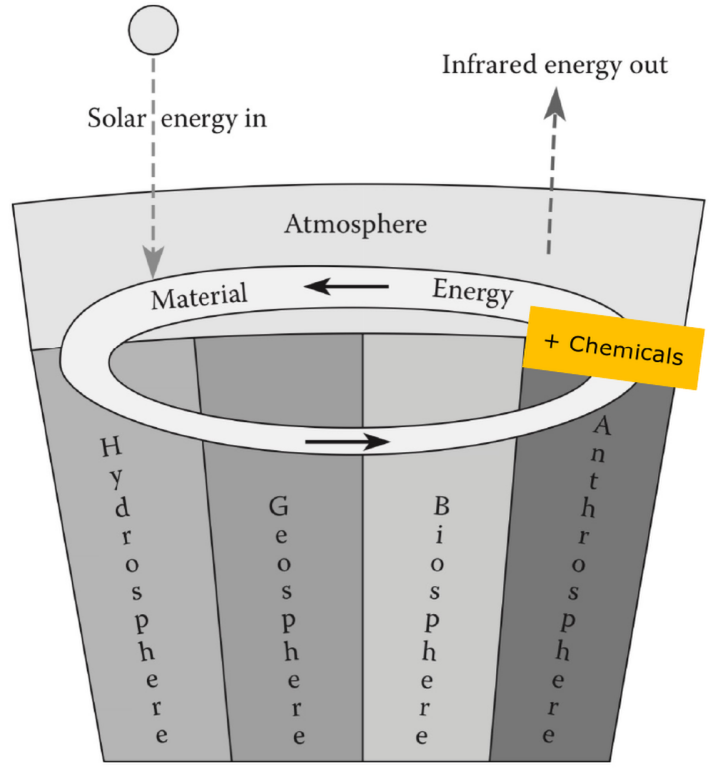
\includegraphics[width=.4\textwidth]{media/earth-system7.png}
\end{wrapfigure}

\phantom{}

The Earth system is essentially a closed system with respect to matter, which circulates
within the five spheres of the environment. Energy enters the Earth system in the form of
sunlight and leaves primarily as infrared radiaton. The balance between these two flows
largely determines Earth's climate and conditions leading to the Antrhopocene.

\defs{The Antrhopocene epoch is an unofficial unit of geologic time, used to describe the
    most recent period in Earth's history when human activity started to have a significant
    impact on the planet's climate and ecosystems.}
\wrapfill
\vspace*{-3cm}

\newpage
\subsection{5-key aspects of pollutants}
\cfig{\includegraphics*[width=\textwidth]{media/pollutant aspects.png}}

Hazardous materials amost always originate in the anthrosphere, are often discarded into
the geosphere, and are frequently transported through the hydrosphere or the atmosphere.
The great concern for their effects is usually on the biosphere, particularly humans beings.

To understand the effect of a chemical in its entirety, it is important to look at the following
5 steps:
\begin{enumerate}
    \item Origin: source of the chemical or pollutant;
    \item Transport: distribution of the pollutant;
    \item Reactions: trasformation of the pollutant;
    \item Effects: impact of the pollutant;
    \item Fate: whereabouts of the pollutant.
\end{enumerate}

\wrn{as long as the pollutant is not completely degraded or remover, the whole cycle
    can/will start again}

\section{Important pollutant categories}
\subsection{Heavy metals}
Heavy metals are material with very high densities.

\subsubsection{Sources}
\begin{itemize}
    \item Pb: lead-acid batteries, lead-bases paints, leaded gasoline;
    \item Hg: coal burning, mining, industrial processes.
\end{itemize}

\subsubsection{Reactions}
\begin{itemize}
    \item Pb, Hg: strong affinity to sulfur (S) \textrightarrow\ bind to enzymes (proteins),
        controlling metabolic reactions;
    \item Hg: bacteria (in water and soil) transform it into CH$_3$Hg$^+$ \textrightarrow\ H$_3$C \textbf{--} Hg$^+$ X$^-$.
\end{itemize}

\subsubsection{Effect}
\begin{itemize}
    \item Hg and Pb damage several organs, mainly the central nervous system;
    \item developmental disorders.
\end{itemize}

\subsubsection{Fate}
\begin{itemize}
    \item persistent in the environment \textrightarrow\ bioaccumulation / biomagnification.
\end{itemize}

\subsection{Greenhouse gases (GHGs)}
GHGs are gases which reflects UVs, impeding them to exit from the ozone
and therefore dissipate their heat in it.

\cfig{\includegraphics*[width=.8\textwidth]{media/Treibhauseffekt-Graphik.jpg}}

\subsubsection{Sources}
\begin{itemize}
    \item CO$_2$: fossil fuels, deforestation \quad \fbox{\chemfig{O=C=O}}
    \item CH$_4$: production of fossil fuels, livestock \quad \fbox{\chemfig{C(-[:-135]H)(<[:-60]H)(<:[:-15]H)(-[:90]H)}}
    \item N$_2$O: agricultural and industrial activities \quad
        \fbox{\rule[-1ex]{0pt}{4.5ex}\schemestart \chemfig{N~\chemabove{N}{+}-O^{-}} \arrow{<->} \chemfig{^{-}N=\chemabove{N}{+}=O}\schemestop}
\end{itemize}

\subsubsection{Reactions}
\begin{itemize}
    \item N$_2$O and CO$_2$ are not reactive;
    \item CH$_4$ can oxide to CO$_2$ and H$_2$O over time.
\end{itemize}

\subsubsection{Effect}
\begin{itemize}
    \item absorb an re-emit infrared radiation \textrightarrow\ global warming / climate change;
    \item Global Warmint Potential (GWP) \textrightarrow\ N$_2$O $>$ CH$_4$ $>$ CO$_2$.
\end{itemize}

\subsubsection{Fate}
\begin{itemize}
    \item atmospgeric persistence:
        \begin{itemize}
            \item CO$_2$ centuries;
            \item N$_2$O: 120 years;
            \item CH$_4$: 12 years.
        \end{itemize}
\end{itemize}

\newpage
\subsection{Particulate matter (PM)}
PM is made by microscopic particles which can depositate inside the
respiratory system of animals and create health problems, such as asthma
or cardiovascular issues.

\subsubsection{Sources}
\begin{itemize}
    \item PM$_{2.5}$ (fines particles): combustion primary, reaction of gases in the atmosphere secondary;
    \item PM$_{10}$: construction sites, road dust, agricolture.
\end{itemize}

\subsubsection{Reactions}
\begin{itemize}
    \item SO$_2$ or NO$_2$ can retract to particulate ammonium sulfate (NH$_4$)$_2$SO$_4$ /
        -nitrate NH$_4$NO$_3$;
    \item the surface of PM facilitates chemical reactions (e.g.: SO$_2$ \textrightarrow\ H$_2$SO$_4$ in water droplets).
\end{itemize}

\subsubsection{Effect}
\begin{itemize}
    \item $\geq$ PM$_{2.5}$: respiratory disease (asthma, COPD);
    \item $\leq$ PM$_{2.5}$: cardiovascular issues (heart attacks, strokes);
    \item chronic exposure: lunge cancer, premature death.
\end{itemize}

\subsubsection{Fate}
\begin{itemize}
    \item atmospheric dispersion (long distances);
    \item deposition (soil, water, vegetation);
    \item bioaccumulation ($\geq$ PM$_{2.5}$).
\end{itemize}
\vspace*{.5cm}
\figbox{\includegraphics*[width=.8\textwidth]{media/particulate-matter.png}}

\newpage
\subsection{Persistent organic pollutants (POPs)}
POPs are chemicals which have a very long degradation time. They are called
``forever chemicals''.

\subsubsection{Halogenated organic compounds (HOCs)}
\pph{Example:} Polychlorinated biphenyls (PCBs);

\pph{Source:} Insulation material (transformers, capacitors), and plastic (until 1979).

\subsubsection{Per- and Polyfluoroalkyl substances (PFASs)}
\pph{Example:} Perfluorooctanoic acid (PFOA);

\pph{Source:} Production of non-stick cookware (Teflon), water-resistant textiles (Gore-Tex)
until 2013/14.

\subsubsection{Both categories}
\begin{itemize}
    \item Reactions: chemically highly stable;
    \item Effect: toxicity (liver, endocrine disruptor), carcinogenity, developmental issues;
    \item Fate: bioaccumulation / biomagnification, can travel long distancies via air and water.
\end{itemize}

\subsubsection{POPs examples}
\pph{PCB No. 77}
\begin{center}
    \chemfig{Cl-*6(-(-[:-120]Cl)=-(-*6(-=-(-Cl)=(-[:60  ]Cl)-=))=-=)}
\end{center}

\pph{PFOA}
\begin{center}
    \chemfig{F-[:-30](-[:-120]F)(-[:-60]F)(-[:30](-[:135]F)(-[:45]F)(-[:-30](-[:-120]F)(-[:-60]F)(-[:30](-[:135]F)(-[:45]F)(-[:-30](-[:-120]F)(-[:-60]F)(-[:30](-[:135]F)(-[:45]F)(-[:-30](-[:-120]F)(-[:-60]F)(-[:30](=[:90]O)(-[:-30]OH))))))))}
\end{center}

\newpage
\subsection{Chlorofluorocarbons (CFCs)}
CFCs are man-made chemical compounds consisting of chlorine, fluorine, and carbon.

\subsubsection{Sources}
\begin{itemize}
    \item refrigerants ( air conditioners and refrigerators);
    \item aerosol propellants (historically);
    \item foam-blowing agents;
    \item industrial solvents.
\end{itemize}

\subsubsection{Reactions}
\begin{itemize}
    \item highly stable in troposphere;
    \item breakdown by UV light in stratosphere;
    \item release of Cl-atoms, leading to ozone depletion.
\end{itemize}

\subsubsection{Effect}
\begin{itemize}
    \item non-toxic;
    \item ozone depletion, Cl-atoms catalyze;
    \item increased UV radiation of Earth's surface.
\end{itemize}

\subsubsection{Fate}
\begin{itemize}
    \item very persistent;
    \item global transport in the atmosphere;
    \item long atmospheric lifetime, between 50 and 100 years.
\end{itemize} 

\subsubsection{CFCs examples}
\pph{CFC-11 (Freon-11)}
\begin{center}
    \chemfig{C(-[:90]F)(-[:-135]Cl)(<[:-60]Cl)(<:[:-15]Cl)}
\end{center}

\pph{CFC-12 (Freon-12)}
\begin{center}
    \chemfig{C(-[:90]Cl)(-[:-135]F)(<[:-60]F)(<:[:-15]Cl)}
\end{center}

\newpage
\subsection{Polycyclic aromatic hydrocarbons (PAHs)}
PAHs are gases created by incompleted combustions, such as tobacco smoke
or grilled food.

\subsubsection{Sources}
\begin{itemize}
    \item incomplete combustion;
    \item tobacco smoke;
    \item grilled/smoked food.
\end{itemize}

\subsubsection{Reactions}
\begin{itemize}
    \item chemically relatively stable;
    \item can partially be degraded by sunlight / microbial activity.
\end{itemize}

\subsubsection{Effect}
\begin{itemize}
    \item toxicity: skin, respiration, immune system;
    \item carcinogens: lung, skin cancer;
    \item developmental issues.
\end{itemize}

\subsubsection{Fate}
\begin{itemize}
    \item persistence (depending on the size);
    \item bioaccumulation / biomagnification;
    \item transport over long distances via air and water.
\end{itemize}

\subsubsection{PAHs examples}

\pph{Naphtalene (Naphta)}
\begin{center}
    \chemfig{*6(=-(*6(=-=-=))--=-)}
\end{center}

\pph{Coronene}
\begin{center}
    \chemfig{*6(-(*6(=-=-))-(*6(=-=-))-(*6(=-=-))-(*6(=-=-))-(*6(=-=-(-[:-90](=[:-30](-[:30])))(=[:28])))-)}
\end{center}

\newpage
\subsection{Volatile organic compounds (VOCs)}
VOCs are gases with a low molecular weight which can evaporate at room temperature.

\subsubsection{Sources}
\begin{itemize}
    \item fossil fuel, fuel storage;
    \item tobacco smoke;
    \item solvent use consumer products (paints, cleaning agents).
\end{itemize}

\subsubsection{Reactions}
\begin{itemize}
    \item VOCs react with NO$_x$ + sunlight to ground-level ozone (O$_3$);
    \item oxidation: reaction with OH, NO$_3$ or O$_3$.
\end{itemize}

\subsubsection{Effect}
\begin{itemize}
    \item toxicity (acute): respiration, headache, dizziness;
    \item toxicity (chronic): liver, kidney, central nervous system;
    \item carcinogens;
    \item developmental issues (certain VOCs).
\end{itemize}

\subsubsection{Fate}
\begin{itemize}
    \item volatility, easily evaporate into the atmosphere;
    \item degradation (photochemical / oxidation processes);
    \item transport over long distances via air.
\end{itemize}

\subsubsection{VOCs examples}

\pph{Toluene}
\begin{center}
    \chemfig{*6(-=-=(-[:90]CH_{3})-=)}
\end{center}

\pph{Benzene}
\begin{center}
    \chemfig{[:30]*6(=-=-=-)}
\end{center}

\pph{Formaldehyde}
\begin{center}
    \chemfig{C(-[:-30]H)(-[:-150]H)(=[:90]O)}
\end{center}

\newpage
\subsection{Environmentally persistent pharmaceutical pollutants (EPPPs)}
EPPPs are pharmaceutical chemicals with a complex structure, which gives to
molecules a big stability and a slow biodegradability.

\subsubsection{Sources}
\begin{itemize}
    \item human and veterinary use;
    \item pharmaceutical waste water.
\end{itemize}

\subsubsection{Reactions}
\begin{itemize}
    \item designed to be chemically stable and bioactive.
\end{itemize}

\subsubsection{Effect}
\begin{itemize}
    \item toxicity (chronic): reproductive, developmental and behavioral effects in acquatic and terrestrial organisms;
    \item antimicrobial resistance;
    \item endocrine disruption.
\end{itemize}

\subsubsection{Fate}
\begin{itemize}
    \item persistence;
    \item bioaccumulation / biomagnification;
    \item can travel through water systems far from the source;
    \item removal inefficiency (waste water treatment plants).
\end{itemize}

\subsubsection{EPPPs examples}

\pph{Ethinylsetradiol}


\pph{Diclofenac (Voltaren)}

\newpage
\subsection{Plastics}
Plastic are synthetics materials made from polymers, long chains of molecules typically
derived from petroleum or natural gas.

\subsubsection{Sources}
\begin{itemize}
    \item production and manufacturing;
    \item consumer use and disposal;
    \item industrial waste;
    \item agricoltural use.
\end{itemize}

\subsubsection{Reactions}
\begin{itemize}
    \item chemically highly stable;
    \item photodegradation limited: breakdown by sunlight \textrightarrow\ microplastics.
\end{itemize}

\subsubsection{Effect}
\begin{itemize}
    \item physical harm: ingestion, entanglement \textrightarrow\ starvation;
    \item chemical exposure: release of toxic additives (phthalates, bisphenol A) \textrightarrow\ endocrine disruptors;
    \item habitat disruption.
\end{itemize}

\subsubsection{Fate}
\begin{itemize}
    \item microplastic formation ($<$ 5mm) \textrightarrow\ found everywhere;
    \item bioaccumulation / biomagnification;
    \item transport by wind, water and ocean currents \textrightarrow\ widespread.
\end{itemize}

\subsubsection{Plastics examples}

\pph{Polyethylene (PE)}
\begin{center}
    \chemfig{\vphantom{C}-[@{op,.75}]C(-[:90]H)(-[:-90]H)-C(-[:90]H)(-[:-90]H)-[@{cl,0.25}]}
    \polymerdelim[height = 35pt, depth = 35pt, indice = {\!\! n}]{op}{cl}
\end{center}

\pph{Polymer chains}




\end{document}
